%===================================================================================================
%  Chapter : 関数
%  説明    : 関数の考え方を確認する.
%===================================================================================================

%   %==========================================================================
%   %  Section : 集合
%   %==========================================================================
        \section{集合}
%       %----------------------------------------------------------------------
%       %  Input
%       %    File Name : PhysNote_Math_Function_Set.tex
%       %    説明      : 素朴な集合論を考える(公理的には扱わない)
%       %----------------------------------------------------------------------
        %   %==========================================================================
%   %  Section : 集合
%   %==========================================================================
        %==================================================================
        %  SubSection
        %==================================================================
            \subsection{集合を定義するとは}
                数学において,\textbf{集合} とは,その最も基礎にあたる概念である.
                数学の要である自然数も,集合という概念を使って定義されるものである.
                自然数の定義は,\textbf{ペアノ
                    \footnote{
                        Giuseppe Peano(1858--1932, イタリア):数学者.自然数を作り出
                        す仕組みである「ペアノの公理系」を提案する.
                    }
                の公理系}として知られている
                    \footnote{
                        ここでは,集合の重要性を示すことが目的なので,
                        ペアノの公理は解説しない.
                        ペアノの公理系を解説するWebサイトは非常に多いし,
                        整数論などの数学の教科書には必ず記述されているので,
                        それらを参照してもらいたい.
                    }.

                集合が数学の最も基礎的な概念であるだけに,それを定義することは
                非常に難しい.中学校や高校で集合について学習するとき,次のように
                集合という概念が説明される.
                    \begin{description}
                        \item[中学・高校での集合の定義] 「集合とは,モノの集まりである.
                        ただし,ここで言うモノとは,集合に属するか否かを明確に判断できる
                        ものに限る.」
                    \end{description}

                この集合の定義は,直観的で非常に分かりやすい.しかし,この“ただ
                し”以下の部分に問題がある.“モノが集合に属すか否かを明確に判断
                できる”とは,どういうことか.「自然数」や「有理数」などは,明確な
                判断が下せるので,モノである.しかし,「美人」とか「厳密」だとか
                というのは,万人に対して明確な判断基準を与えることができず,モノ
                ではありえない.となると,どういった場合に,モノになりうるのかと
                いう疑問が自然と脳裏にうかんでくる.しかし,実際問題として,モノ
                になりうるかどうかの判断基準を明示することは不可能なのである.
                つまり,「モノの集まりを集合という」といった集合の定義は,深く考
                えると曖昧な部分が浮き彫りにされてくるのである
                    \footnote{
                        \textbf{集合論が含む矛盾}\;\;\;たしかに,集合論(特に無限集合論)
                        の開拓者であるカントール
                        (※1)が与えた集合の定義は「モノの集まりを集合という」であった.
                        しかし,この定義を用いると,矛盾したことが起こってしまうことをラッセル(※2)が
                        発見した.この矛盾したこととは,次のような命題(定義A)を考える
                        ことで説明される.
                        \begin{itemize}
                            \item
                                \textbf{定義A}:「自分自身を含まない全ての集合を $\omega$ とする」
                        \end{itemize}

                        さて,どこが矛盾なのかを説明しよう.次の問題を考えてみる.
                        \begin{itemize}
                            \item
                                \textbf{問題X}:「$\omega$ は,$\omega$ 自身に含まれるか,否か」
                        \end{itemize}

                        考えらる答えは2つしかない.1.)含まれるか,2.)含まれないか,のどちらか
                        である.さて,1.)の状況,つまり,$\omega$ は $\omega$ 自身に含まれる
                        と仮定しよう.この場合,定義Aにより自分自身を含まない.しかし,いま,
                        $\omega$ 自身に含まれているという仮定に反する.つまり,「1.)含まれる」
                        は間違いである.では,2.)の状況,つまり,$\omega$ は $\omega$ 自身に含
                        まれないが答えなのだろうか.しかし,この場合,定義Aに反していることは明
                        白であり,「2.)含まれない」も間違いである.考えられるすべての答えで前提
                        とする条件と矛盾する結果がでてしまう.これを \textbf{ラッセルのパラド
                        クス} という.どう考えても,定義Aによって作られる集合 $\omega$ は問題Xを
                        突きつけられると,その答えは矛盾を生じるという結果に終わる.

                        これは致命的な問題である.集合はすべての数学の分野の基礎にあたる概念で
                        あり,この部分に欠陥があるということは,すべての数学分野の存立が危うく
                        なる.

                        ここで示した矛盾以外以外にも,カントール自身が発見した \textbf{カントー
                        ルのパラドクス} がある.任意の集合 $A$ に対し,それよりも大きい集合を
                        作成できることが証明されている(「集合の集合」を考えることができてしまうので).
                        にもかかわらず,最大の大きさを持つ集合
                        があることも証明されてしまった.つまり,いくらでも大きい集合を考えること
                        ができると保証されているのに,その大きさには上限があるという.明らかに,
                        矛盾している.(自然数を例として言えば,「自然数はいくらでも大きい数を創
                        りだすことができるのに,それには最大値がある」と言っているのと同じである)

                            (※1)カントール:Georg Ferdinand Ludwig Philipp Cantor(1845--1918, ロシア)

                            (※2)ラッセル:Bertrand Arthur William Russell(1872--1970, イギリス)
                    }.

                どう定義したものか.答えを先に書いてしまうと,実は,
                数学的に厳密に集合を直接定義することはできないのである.集合は数学
                的に言えば,\textbf{無定義語} として扱われる概念なのである.

                通常,数学
                では,ある概念を定義する場合,既存の概念を基にする.しかし,数学も
                言葉を使う以上,「言葉のもつ限界」をふくんでしまう.ここで言葉のも
                つ限界と表現したのは,ある単語を説明するには,他の別の言葉を用いな
                ければならないということである.これの何が限界なのかといえば,次の
                例を考えればよい.例えば,「全体」という語彙が“全ての部分”という
                ように定義されているとしよう.では,この定義で出てくる「部分」とは
                何か.部分の定義はどうしたらよいかを考えても,“部分とは全体を複
                数個に分割したものの中の,その1つのこと”というような表現になってし
                まう.この部分の定義には,「全体」という語彙が含まれているが,一方
                で全体の定義では「部分」という語彙が使用されている.つまりは,語彙
                の定義が循環してしまっているのである.もっと抽象的に言えば,次の2つ
                の定義が同時になされているということである.
                    \begin{description}
                        \item[\;\;\;定義 {\rm P}:\;]
                            AとはBであることをいう.
                        \item[\;\;\;定義 {\rm Q}:\;]
                            BとはAであることをいう.
                    \end{description}
                こうなると,定義Pを行うには,それに先立って定義Qがなされていなければ
                ならなし,しかし,定義Qをするには,それに先立って定義Pがなされていな
                いといけない.定義が堂々巡りしてしまうのである.これでは数学的に厳密
                な議論ができない.集合を通常通り数学的に厳密に定義しようとするとき,
                このような限界から,その実行は不可能であると言わざるをえない.

                では,どうすればよいか.これには選択肢が次の2つ考えられる.
                    \begin{enumerate}
                        \item 集合を無定義語として扱う(集合を公理的に定義する)
                        \item 数学的厳密性を犠牲にする
                    \end{enumerate}

                まず選択肢1から説明しよう.
                無定義語とは,このような言葉の限界を回避すべく考え出された解決策である.
                驚くべきことに
                    \footnote{
                        「無定義語」という語彙から,推察されてしまい,驚かないかも
                        しれない.しかし,それでも革命的な考え方であると感じること
                        と思う.
                    },
                無定義語とは,数学的に直接定義されないのである.では,どう説明されるのか.
                この考え方は盲点だったかもしれない.次のようになされる.例えば,
                Aという概念を定義したいが,数学的に厳密に定義しようとするとき,言葉の限界
                からそれが不可能であることが判明したとする.しかし,今定義したいAという概
                念のもつ性質は十分に考えられているとしよう.このとき,概念Aを定義するには,
                最初に,その性質を必要十分であるように,列挙する.ここで挙げられる性質
                は複数個になることだろう.そして,この複数個の性質を満たすものをAと定義
                するのである.これを実行すると次のようになるだろう.
                    \\
                    \begin{itembox}[l]{\textbf{無定義語Aの説明の仕方}}
                        以下の性質をもつものをAという.
                        \begin{enumerate}
                            \item Aには,性質 X${}_{1}$ が備わっている.
                            \item Aには,性質 X${}_{2}$ が備わっている.
                            \item Aには,性質 X${}_{3}$ が備わっている.
                            \item …(以下,いくつか続く)
                        \end{enumerate}
                    \end{itembox}
                    \\

                もちろん,このように説明される概念Aには,日常的な意味を考えると
                直感的イメージにそぐわない,複数のものが想像されてしまうかもしれ
                ない.しかし,数学的には,それらすべてを区別することはせず,同一
                視するのである.なぜかといえば,語彙Aは無定義語Aということを示す
                記号に過ぎず,その意味などは一切考慮されないからである.無定義語
                Aが他の概念と区別できれば良いのである.無定義語の例として,「点
                」・「直線」などが有名であるが,これらは「点」,「直線」と表現し
                なければならないわけではない.一貫して同一の語彙を使用していれば,
                同表現してもかまわないのである.ヒルベルト
                    \footnote{
                        ヒルベルト(David Hilbert, 1858--1932, ドイツ):数学者.
                        整数論,数学基礎論,積分方程式論など広い分野にわたり,著しい
                        功績がある.また,ヒルベルト空間など,物理学への貢献も多く
                        ある(物理学の公理化も目論でいたらしい).

                        (参照)Constance Reid[著],彌永健一[訳],『ヒルベルト---現代数学の巨峰』
                    }
                が言ったとされる,「机と椅子とビールジョッキの幾何学」という表現
                は,このことである.点を「机」と言い換え,直線を「椅子」と言い換えても,
                数学的には何の支障もない
                    \footnote{
                        こう言うと,無定義語にはAやBというように抽象的な記号を割り
                        当てよう,という考え方が生まれてしまうかもしれない.
                        しかし,だからと言って,不用意に記号化することは好ましくない.
                        数学は人間がその想像力により発展させるものであり,そのためには
                        イメージが非常に重要である.イメージによりインスピレーションが
                        湧き,数学が発展するのである.安易に無定義語を記号化してしまうと,
                        イメージすることが難しくなってしまう.なので,無定義語にはできる
                        限り,イメージしやすい語彙を割当てるべきなのである.点という語彙
                        から意味を削ぎ落とされたとしても,点というイメージを捨て去るべき
                        ではないということである.
                    }.

        %==================================================================
        %  SubSection
        %==================================================================
            \subsection{集合の直感的定義}
                前節では,集合を数学的に厳密に扱うべく,無定義語という考え方を紹介
                した.しかし,ここでは物理学を学習しているのであって,厳密な数学を
                理解しようとしているのではないのだから,集合の定義に無定義語という
                概念を持ち出して話を難しくしたくない.そこまで数学的な厳密性にこだ
                わる必要もないので,ここでは,集合を直感的に定義して扱っていきたい.
                このような考え方は,素朴集合論といわれている.高校数学における集合
                とは,素朴集合論である.このノートでも,以下では集合といえば,素朴
                に定義された集合のであるとする.

                集合の素朴な定義は,次のようになされる.
                    \begin{myshadebox}{直感的な集合の定義}
                        \begin{dfn}\label{dfn:set}
                        “もの”の集まりのことを \textbf{集合} という.
                            \begin{description}
                                \item[記号] 集合を表現するのには,多くの教科書
                                では,大文字のアルファベットが用いられる.例えば,
                                    \begin{equation*}
                                        \mbox{集合 A}
                                    \end{equation*}
                                のように.このノートでも,この表現を採用する.
                            \end{description}
                        \end{dfn}
                    \end{myshadebox}

                ここでいう“もの”とは何でもよいということではなく,
                数学的に厳密に扱えるものでないといけない.例えば,「美しいものの集合」
                といわれても,これは数学的に扱うことはできない.「美しい」という定義が
                曖昧だからだ.数学的に扱える集合とは,例えば自然数や整数があげられよう.

        %==================================================================
        %  SubSection
        %==================================================================
            \subsection{集合の要素}
                「集合」と言うからには,その中には,何らかの構成要素があるは
                ずである.というか,そういうもの想定して,集合を定義している.
                そこで,集合を構成するものの呼び方を与えておく(定義\ref{dfn:set_elements}).
                また,後の学習で要素について考えるときに,例えば,
                ある概念 $a$ がその集合 $A$ の要素であることを数式的に示せると,
                便利である.
                \\
                \begin{itembox}[l]{\textbf{集合の要素}}
                    \begin{dfn}\label{dfn:set_elements}
                        集合を構成するもの
                            \footnote{
                                例えば上の1から5の自然数の集合 $A$ であれば,1,2,3,4,5
                                の5つの自然数である.
                            }
                        を集合の \textbf{要素} という
                            \footnote{
                                元(げん)ということもある.教科書によって様々なよび方がなされ
                                る.
                            }.
                        \begin{description}
                            \item[記号] ある要素 $a$ が集合 $A$ に含まれているということを,
                                \begin{equation*}
                                    a\ni A.
                                \end{equation*}
                            と記述する.これは左右を逆転させて
                                \begin{equation*}
                                    A \in a.
                                \end{equation*}
                            と表現しても同じことである.
                        \end{description}
                    \end{dfn}
                \end{itembox}
                \\


        %==================================================================
        %  SubSection
        %==================================================================
            \subsection{空集合の存在:$\emptyset$}
                集合は要素を含むつことが一般的だ.
                しかし,「要素を全く含まない集合」という
                ものも考えられる.それについて,次に説明しよう.

                要素をひとつも含まない集合を,\textbf{空集合}
                    \footnote{
                        空集合:「くうしゅうごう」と読む.「そらしゅうごう」
                        でも「からしゅうごう」でも「あきしゅうごう」でもないよ.
                    }
                という.

                空集合には要素がないのだけど,これを表現したい場合
                もある.そのために,$\emptyset$ という記号を使うことが一般
                的である.このノートでも,この記号 $\emptyset$ を用いる
                    \footnote{
                        空集合を表す記号 $\emptyset$ は,“数字の0に斜め線をいれ
                        た記号”である.よく,ギリシャ文字の $\phi$ が使われている
                        ことがあるが,これは間違いである.フォントが足りなかった
                        時代の古い教科書では,$\phi$ を $\emptyset$ の代わりとし
                        て使用されていることもあるので,注意が必要.ノートをとる
                        時に,$\phi$ と見分けが付かなくなることもあるが,イメージ
                        は $\emptyset$ であることを意識すること.
                    }.
                つまり,空集合の要素は次のように表現できる
                    \footnote{
                        ここで用いられる記号 $\emptyset$ には,「空っぽである」
                        というイメージが込められている.
                    }.
                    \begin{equation*}
                        A \in \emptyset.
                    \end{equation*}
                「空集合は空っぽの要素をもつ」と言い換えられるのである
                    \footnote{
                        何かまわりくどい言い回しであるが,こう表現することで,
                        数学体系をより豊かにできるのである.まあ,こ
                        こでは物理のための数学を学習しているので,どんな風に豊か
                        になるかには興味はない.詳細は,集合論の教科書を参照
                        してほしい.
                    }.

                    改めて,定義しておこう.
                    \\
                    \begin{itembox}[l]{\textbf{空集合の存在}}
                        \begin{dfn}
                            要素をひとつも含まない集合を \textbf{空集合} という.
                            \begin{description}
                                \item[記号] 集合Aが空集合であるとは,次のように表現される.
                                \begin{equation*}
                                    A \in \emptyset.
                                \end{equation*}
                            \end{description}
                        \end{dfn}
                    \end{itembox}
                    \\

                    ここに用いられる記号 $\emptyset$ には
                    「空っぽ」であるという意味が込められている.

        %==================================================================
        %  SubSection
        %==================================================================
            \subsection{ある集合を定義する}
            %==================================================================
            %  SubsubSection
            %==================================================================
                \subsubsection{特別な集合の定義の表現方法}
                    ある特別な集合を定義
                        \footnote{
                            ここで,ひとつ断っておかないといけないことがある.今
                            までは単に「集合の定義」という言葉を使っていたが,こ
                            れには次のような2通りの意味が考えられる.ひとつは,1.)
                            集合という概念そのものの定義という意味である.もうひ
                            とつは,2.)要素が限定されている集合を定義する場合であ
                            る.1の場合の例は上げるまでもない.2の場合の例をあげよ
                            う.例えば,要素が自然数のみの集合を考えたい場合,
                            「集合 $\bN$ を自然数の集合とする」という.
                            この場合は,集合の概念そのものの定義ではなく,ある性質を
                            持った特別な集合を考えたい場合に,ある記号をその集合に割
                            り当てるという,集合の定義である.

                            このように,「集合の定義」という言葉には2通りの意味が考え
                            られるが,これらの違いは文脈上で峻別できることである(多く
                            の場合,2の場合の意味である).
                        }
                    したい場合,その表現は次の2種類ある.その記述例と特徴を説明する.
                        \\
                        \begin{itembox}[l]{\textbf{ある集合の定義の方法}}
                            \begin{enumerate}
                                \item \textbf{内包的定義}
                                    \begin{itemize}
                                        \item[例.)] $A=\{ x \,| \, x \mbox{は偶数} \}$
                                        \item 要素の持つ性質を,式等を用いて集合を定義する方法.
                                        \item 要素の個数が無限にあっても記述可能である.
                                        \item 要素の具体例がすぐにイメージしづらいことも多い.
                                    \end{itemize}
                                \item \textbf{外延的定義}
                                    \begin{itemize}
                                        \item[例.)] $A=\{ \,1,\,2,\,3,\,4,\,5\,\}$
                                        \item 集合のもつすべての要素を列挙して集合を定義する方法.
                                        \item 要素の個数が無限であると,表現しきれない場合がある.
                                        \item 要素の具体例は,直接記述されているので,イメージしやすい.
                                    \end{itemize}
                            \end{enumerate}
                        \end{itembox}
                        \\
                    以下で,もう少し詳しく説明する.

            %==================================================================
            %  SubsubSection
            %==================================================================
                \subsubsection{集合の内包的定義}
                    内包的定義とは,その集合のもつ性質を表して集合を定義する
                    というものである.例えば,「偶数の集合 $A$ 」を表現するには,
                                \begin{equation*}
                                    A=\{ x \,| \, x \mbox{は偶数} \}
                                \end{equation*}
                    と書く.一般には,この例で「$x$ は偶数」の部分を $P(x)$ と表現して,
                                \begin{align}
                                    A=\{\underbrace{ x }_{\mbox{変数}}|\underbrace{ P(x) }_{\mbox{条件式}}\}
                                \end{align}
                    と書く
                        \footnote{
                            この $P(x)$ は \textbf{述語} とよばれる.ここら辺は,論理学等
                            の教科書を読んでみよう.ここでは深く考えずに話を先へ進める.
                        }.
                    読み方としては,「条件 $P(x)$ を満たすような $x$ の集合」といったカン
                    ジである.

                    \begin{memo}{注意}
                        ここに書いた「変数」というのは,要素を一般的に表現する変数の
                        ことである.
                    \end{memo}

            %==================================================================
            %  SubsubSection
            %==================================================================
                \subsubsection{集合の外延的定義}
                    外延的定義とは,その集合を構成する要素全てを列挙して,その
                    集合を表現するというものである.例えば1から5までの自然数の集合は
                        \begin{equation*}
                            A=\{\underbrace{\,1,\,2,\,3,\,4,\,5\,}_{\mbox{要素の列挙}}\}
                        \end{equation*}
                    と書く.これはまた,内包的にも表現できて,
                        \begin{equation*}
                            A=\{\underbrace{ x }_{\mbox{変数}}|\underbrace{ 1\leq x\leq 5,\; x\mbox{は自然数} }_{\mbox{条件式}}\}
                        \end{equation*}
                    と書ける.外延的定義は集合の要素に規則性がないときに用いることが多い.
                    また,内包的定義よりも直感的にわかりやすいならば,外延的定義が
                    用いられることもある.しかし概して,一般的には内包的定義のほうがよく用
                    いられるようである.




        %==================================================================
        %  SubSection
        %==================================================================
            \subsection{集合の性質}
                実数を扱う場合には,等号や不等号といった,
                右辺と左辺の関係を表現する必要があった.集合にもこれと同等
                な概念がある.それは,次のようなものである.これらについて,
                詳細は次節以降で考える
                    \footnote{
                        ここではとりあえず,このような概念
                        があるということを認識できれば,それで良い.
                    }.
                \\
                \begin{itembox}[l]{\textbf{複数の集合の間の関係}}
                    2つ以上の集合が存在するとき,それらの集合同士の
                    間に,次のような関係が定義される.
                        \begin{itemize}
                            \item 包含関係(部分集合)
                            \item 二項関係
                            \item 同値関係
                        \end{itemize}
                \end{itembox}
                \\

                また,今まで親しんできた実数の加法・乗法などの演算のように,
                集合も演算の対象となることができる.しかし,集合の演算
                は,加法・乗法という言葉は使われない.実数の意味での加法・
                乗法と少々異なるからである.
                集合の代表的な演算の種類は次の通りである.
                \\
                \begin{itembox}[l]{\textbf{集合の演算的性質}}
                    2つ以上の集合が存在するとき,それらの集合に対し,
                    以下のような概念が定義される.
                        \begin{itemize}
                            \item 共通部分
                            \item 合併集合(または,和集合)
                            \item 補集合
                            \item 差集合
                            \item 直積(または,積集合)
                            \item 商集合
                            \item 冪集合
                                \footnote{
                                    冪集合:「べきしゅうごう」と読む.$a^{x}$ のような
                                    指数で表される積のことをいう.
                                }
                        \end{itemize}
                \end{itembox}
                \\



            %==================================================================
            %  SubsubSection
            %==================================================================
                \subsubsection{集合の共通部分}
                    2つの集合を用意しよう.要素は任意のものでよい.この適当な2つの
                    集合を $A$,$B$ と表すことにする.このとき,集合 $A$ と集合 $B$ の
                    の両方の集合において,それぞれの要素を考えると,次のものがある.
                        \begin{enumerate}
                            \item 集合 $A$ のみに属し,かつ,集合 $B$ には属さない要素
                            \item 集合 $B$ のみに属し,かつ,集合 $A$ には属さない要素
                            \item 集合 $A$ と $B$ の両方に属する要素
                        \end{enumerate}

                    図示すれば,図\ref{fig:kyoutububun1}の様である.
                    集合 $A$ と集合 $B$ の定義の仕方によっては,どちらの集合にも属さない
                    要素の存在も考えられる(図\ref{fig:Kyoutububun1} (B)).
                        \begin{figure}[hbt]
                            \begin{tabular}{cc}
                                \begin{minipage}{0.5\hsize}
                                    \begin{center}
                                        \includegraphicsdouble{kyoutububun1.pdf}

                                        (A)
                                    \end{center}
                                \end{minipage}
                                \begin{minipage}{0.5\hsize}
                                    \begin{center}
                                        \includegraphicsdouble{kyoutububun2_phi.pdf}

                                        (B)
                                    \end{center}
                                \end{minipage}
                            \end{tabular}
                                        \caption{共通部分(例:集合が2つの場合)}
                                        \label{fig:Kyoutububun1}
                        \end{figure}

                    図\ref{fig:Kyoutububun1}の円で囲まれた領域の内側に,
                    その集合の要素が含まれている.ここでは,境界線上の
                    点は含めないこととする.

                    共通部分を示す記号として,$\cap$ が用いられる
                        \footnote{
                            共通部分を表す記号 $\cap$ に正式に決まった名称
                            は与えられていないが,多くの教科書では「キャップ」と
                            い名前が与えられている.
                        }.
                    例えば,集合 $A$ と集合 $B$ の共通部分は,
                        \begin{equation*}
                            A \cap B
                        \end{equation*}
                    というように表現される.


                    もっと一般的に,2個以上の集合を考え,
                    それらの共通部分を図示すると,図\ref{fig:kyoutububun_gen}のようになる.
                    ここでは,4つの集合しか描いていないが,この集合の個数は任意に設定できる.
                        \begin{figure}[hbt]
                            \begin{center}
                                \includegraphicsdefault{kyoutububun_gen.pdf}
                                \caption{共通部分}
                                \label{fig:kyoutububun_gen}
                            \end{center}
                        \end{figure}


                    ここで,集合を添字付きのアルファベットに書きなおした
                        \footnote{
                            これは,アルファベットの種類がAからZの26種類しかないからである.
                            アルファベットのみによる集合の表し方を採用している
                            と,26個までの集合しか区別して扱うことができない.
                            そこで,同じアルファベットでも,添字をつけて区別することで,
                            集合を区別できるようにするのである.こうすると,
                            すぐ後に述べる,複数の集合の共通部分を表す
                            省略記号 $\bigcap_{i=1}^{n}$ の
                            導入も自然に行うことができる.
                        }.
                    この場合,集合の共通部分は
                        \begin{equation*}
                            A_{1} \cap A_{2} \cap A_{3} \cap A_{4}
                        \end{equation*}
                    と表される.

                    同様に,集合の数が $n$ 個の場合は,
                        \begin{equation*}
                            A_{1} \cap A_{2} \cap \cdots \cap A_{n-1} \cap A_{n}
                        \end{equation*}
                    と表される.
                    想定する集合の個数が多くなると,その共通部分の表現も長ったらしく
                    なり,読みづらくなる.そこで,新たに記号を導入することにしよう.
                    次の通りである.
                        \begin{equation*}
                            \bigcap_{i=1}^{n} A_{i}
                                :=  A_{1} \cap A_{2} \cap \cdots \cap A_{n-1} \cap A_{n}
                        \end{equation*}

                    省略記号 $\bigcap_{i=1}^{n}$ により,$i=1$ から $i=n$ まで
                    の集合の共通部分の表現を簡略化できる
                        \footnote{
                                これは,和の記号 $\displaystyle\Sigma_{i=1}^{n}a_{i}$ に
                                真似た記号である.
                        }.

                    集合の個数に上限がないのなら(無限個の集合を想定する場合),
                    個数 $n$ を無量大数を表す記号 $\infty$ に置き換えて,
                        \begin{equation*}
                            \bigcap_{i=1}^{\infty} A_{i}
                                :=  A_{1} \cap A_{2} \cap  A_{3} \cap \cdots
                        \end{equation*}
                    と表現する.

                    ここで,改めて,集合の共通部分を定義しておこう.
                    \\
                    \begin{itembox}[l]{\textbf{集合の共通部分}}
                        \begin{dfn}
                            集合が $n$ 個ある場合を考え,それらを $A_{1}\,,\,A_{2}\,,\,\cdots\,A_{n}$ と
                            する.この $n$ 個の集合全てに属する要素を,
                            これらのすべての集合の \textbf{共通部分} という.
                            \begin{description}
                                \item[記号1] 集合の個数が2つの場合,記号 $\cap$ を用いて,
                                        \begin{align}
                                                A_{1} \cap A_{2}.
                                        \end{align}
                                \item[記号2] 集合の数が2つ以上の場合,その個数を $n$ 個として,
                                        \begin{align}
                                            \bigcap_{i=1}^{n} A_{i}
                                                :=  A_{1} \cap A_{2} \cap \cdots \cap A_{n-1} \cap A_{n}.
                                        \end{align}
                                \item[記号3] 集合の個数に上限をつけない場合,記号 $\infty$ を用いて,
                                        \begin{align}
                                            \bigcap_{i=1}^{\infty} A_{i}
                                                :=  A_{1} \cap A_{2} \cap  A_{3} \cap \cdots\,.
                                        \end{align}
                            \end{description}
                        \end{dfn}
                    \end{itembox}
                    \\

                    特に注意しておこう.想定する全ての集合($A_{1}\,,\,A_{2}\,,\,\cdots\,A_{n}$)の
                    共通部分がないとき,それは共通部分は空集合であると言い換える
                    ことができる.
                    \\
                    \begin{itembox}[l]{\textbf{共通部分がない場合}}
                        想定する複数個の集合に対し,共通部分が存在しない場合,
                        共通部分は空集合であるといい,次の記号で表現できる.
                        \begin{align}
                           \emptyset = \bigcap_{i=1}^{n} A_{i}
                           \quad
                           \Longleftrightarrow
                           \quad
                           \bigcap_{i=1}^{n} A_{i} \mbox{の共通部分なし}.
                        \end{align}
                    \end{itembox}
                    \\

                        \begin{figure}[hbt]
                            \begin{center}
                                \includegraphicsdefault{kyoutububun2_phi.pdf}
                                \caption{共通部分なし $=$ 共通部分は空集合}
                                \label{fig:kyoutububun2_phi}
                            \end{center}
                        \end{figure}


            %==================================================================
            %  SubsubSection
            %==================================================================
                \subsubsection{合併集合(または,和集合)}
                    任意に集合を2つ用意して,それぞれ集合 $A$,集合 $B$ と名付けよう.
                    この2つの集合のもつ要素をあわせて新たに集合を作るとき,これを
                    集合 $A$ と集合 $B$ の \textbf{合併集合} という.
                    図示すれば,図\ref{fig:gappei_shugo1}のように描けよう.
                        \begin{figure}[hbt]
                            \begin{center}
                                \includegraphicsdefault{gappei_shugo1.pdf}
                                \caption{合併集合}
                                \label{fig:gappei_shugo1}
                            \end{center}
                        \end{figure}

                    合併集合は,また \textbf{和集合} ともいわれる.2つの集合より
                    作られる合併集合を表す記号として,$\cup$ が用いられる
                        \footnote{
                            合併集合を表す記号 $\cup$ に正式に決まった名称
                            は与えられていないが,多くの教科書では「カップ」と
                            い名前が与えられている(コーヒーカップとか,マグカッ
                            プとかの“カップ”である).
                        }.

                    例えば,集合 $A$ と集合 $B$ の合併集合は,
                        \begin{equation*}
                            A \cup B
                        \end{equation*}
                    というように表現される.

                    もっと一般的に,2個以上の集合を考え,
                    それらの合併集合を図示すると,図\ref{fig:kyoutububun_gen}のようになる.
                    ここでは,4つの集合しか描いていないが,この集合の個数は任意に設定できる.
                        \begin{figure}[hbt]
                            \begin{center}
                                \includegraphicsdefault{gappei_shugo.pdf}
                                \caption{合併集合}
                                \label{fig:gappei_shugo}
                            \end{center}
                        \end{figure}

                    ここで,集合を添字付きのアルファベットに書きなおした.
                    この場合,集合の合併集合は
                        \begin{equation*}
                            A_{1} \cup A_{2} \cup A_{3} \cup A_{4}
                        \end{equation*}
                    と表される.

                    同様に,集合の数が $n$ 個の場合は,
                        \begin{equation*}
                            A_{1} \cup A_{2} \cup \cdots \cup A_{n-1} \cup A_{n}
                        \end{equation*}
                    と表される.
                    想定する集合の個数が多くなると,その合併集合の表現も長ったらしく
                    なり,読みづらくなる.そこで,新たに記号を導入することにしよう.
                    次の通りである.
                        \begin{equation*}
                            \bigcup_{i=1}^{n} A_{i}
                                :=  A_{1} \cup A_{2} \cup \cdots \cup A_{n-1} \cup A_{n}
                        \end{equation*}

                    省略記号 $\bigcup_{i=1}^{n}$ により,$i=1$ から $i=n$ まで
                    の集合の合併集合の表現を簡略化できる
                        \footnote{
                                これは,和の記号 $\displaystyle\Sigma_{i=1}^{n}a_{i}$ に
                                真似た記号である.
                        }.

                    集合の個数に上限がないのなら(無限個の集合を想定する場合),
                    個数 $n$ を無量大数を表す記号 $\infty$ に置き換えて,
                        \begin{equation*}
                            \bigcup_{i=1}^{\infty} A_{i}
                                :=  A_{1} \cup A_{2} \cup  A_{3} \cup \cdots
                        \end{equation*}
                    と表現する.

                    ここで,改めて,合併集合を定義しておこう.
                    \\
                    \begin{itembox}[l]{\textbf{合併集合}}
                        \begin{dfn}
                            集合が $n$ 個ある場合を考え,それらを $A_{1}\,,\,A_{2}\,,\,\cdots\,A_{n}$ と
                            する.この $n$ 個の集合全てに属する要素を,
                            これらのすべての集合の \textbf{合併集合} という.
                            \begin{description}
                                \item[記号1] 集合の個数が2つの場合,記号 $\cup$ を用いて,
                                        \begin{align}
                                                A_{1} \cup A_{2}.
                                        \end{align}
                                \item[記号2] 集合の数が2つ以上の場合,その個数を $n$ 個として,
                                        \begin{align}
                                            \bigcup_{i=1}^{n} A_{i}
                                                :=  A_{1} \cup A_{2} \cup \cdots \cup A_{n-1} \cup A_{n}.
                                        \end{align}
                                \item[記号3] 集合の個数に上限をつけない場合,記号 $\infty$ を用いて,
                                        \begin{align}
                                            \bigcup_{i=1}^{\infty} A_{i}
                                                :=  A_{1} \cup A_{2} \cup  A_{3} \cup \cdots\,.
                                        \end{align}
                            \end{description}
                        \end{dfn}
                    \end{itembox}
                    \\

                    \begin{figure}[hbt]
                        \begin{center}
                            \includegraphicsdefault{shugo_rei.pdf}
                            \caption{共通部分/合併集合}
                            \label{fig:shugo_rei}
                        \end{center}
                    \end{figure}

            %==================================================================
            %  SubsubSection
            %==================================================================
                \subsubsection{補集合}
                    今までは,例えば集合 $A$ を考えるときに,その外側の領域
                    については,全く考慮していなかった.しかし,集合 $A$ の
                    外側の領域についても考えられるので,それを無視す
                    ることはできない.
                    図で描けば,図\ref{fig:ho_shugo}のようになる.
                        \begin{figure}[hbt]
                            \begin{center}
                                \includegraphicsdefault{ho_shugo.pdf}
                                \caption{補集合}
                                \label{fig:ho_shugo}
                            \end{center}
                        \end{figure}

                    そこで,次のような定義をしよう.
                    \\
                    \begin{itembox}[l]{\textbf{補集合}}
                        \begin{dfn}
                            任意の集合 $A$ の外側の領域に含まれている全ての要素からなる集合
                            を,集合 $A$ の \textbf{補集合} とよぶ.
                            \begin{description}
                                \item[記号1] 集合 $A$  補集合を表す記号として,このノートでは
                                            以下の記号を用いる.
                                                \begin{align}
                                                        A^{c}.
                                                \end{align}
                                             ここで1つ注意がある.
                                             この上付きの添字記号 $c$ は定数ではない.
                                             なので,これを「$A$ の $c$ 乗」というように
                                             解釈してはならない
                                                \footnote{
                                                    補集合を英語で表すと,"a complementary set" で
                                                    あるので,上付き添字の $c$ はこれに由来するので
                                                    はないかと思う.確かではないが.まあ,記号なんて,
                                                    その由来なんか気にする必要なんてないのだけど.
                                                }.
                                \item[記号2] 集合 $A$ の補集合 $A^{c}$ は,「集合 $A$ でない,他の全ての
                                             集合の合併集合」と捉えることができる.簡単に表現すれば,
                                             「集合 $A$ でない集合」となる.この表現は集合 $A$ の否定
                                             であり,ブール代数などでは,
                                                \begin{equation*}
                                                    \bar{A}
                                                \end{equation*}
                                             と書かれることも多い.
                            \end{description}
                        \end{dfn}
                    \end{itembox}
                    \\


            %==================================================================
            %  SubsubSection
            %==================================================================
                \subsubsection{差集合}
                    任意に集合を2つ用意して,それぞれ集合 $A$,集合 $B$ と名付けよう.
                    この2つの集合 $A$,$B$ には空集合でない共通部分が存在すると
                    仮定する.つまり,
                        \begin{equation*}
                            A\cap B \neq \emptyset
                        \end{equation*}
                    を想定する.

                    このとき,次のことを考えられる.それは「集合 $A$ に
                    属している要素のうち,集合 $B$ に属していない全ての要素か
                    らなる集合」である.図で描けば,図\ref{fig:sa_shugo1}のよ
                    うになる.
                        \begin{figure}[hbt]
                            \begin{center}
                                \includegraphicsdefault{sa_shugo1.pdf}
                                \caption{差集合}
                                \label{fig:sa_shugo1}
                            \end{center}
                        \end{figure}

                    改めて定義しておこう.
                    \\
                    \begin{itembox}[l]{\textbf{差集合}}
                        \begin{dfn}
                            任意の2つの集合 $A$,$B$ があるとき,
                            集合 $A$ に属している要素のうち,集合 $B$ に属して
                            いない全ての要素からなる集合のことを,集合 $A$ から
                            集合 $B$ を引いた \textbf{差集合} という.
                            \begin{description}
                                \item[記号]  集合 $A$ から集合 $B$ を引いた差集合を,
                                             このノートでは以下のように記述する.
                                                \begin{align}
                                                        A\setminus B
                                                \end{align}
                                             のようである
                                                \footnote{
                                                    これは,差集合が実数の意味で
                                                    の $-$ とは異なる概念だからだろう.合併集合
                                                    の記号 $\cup$ の記号にしても,同じことがいえよう.

                                                    教科書によっては,差集合を $A-B$ のように表現しているもの
                                                    も見受けられる.しかし,その場合でも,合併集合の
                                                    記号は $\cup$ を採用していることが多い.$+$ にす
                                                    れば良いのに.
                                                }.
                            \end{description}
                        \end{dfn}
                    \end{itembox}
                    \\
            %==================================================================
            %  SubsubSection
            %==================================================================
                \subsubsection{直積(または,積集合)}
                    任意に集合を2つ用意して,それぞれ集合 $A$,集合 $B$ と名付けよう
                        \footnote{
                            この記述,飽きてきたかな.何か別の言い回しで,このマンネリ
                            をなくしたいな.何かいいアイディア,ないかな.
                        }.
                    このとき,次の操作を行うことを考える.集合 $A$ から任意に
                    要素を一つ選択する.これを
                        \begin{equation*}
                            x_{A} \in A
                        \end{equation*}
                    としよう.同様に,集合 $B$ に対してもこの操作を行い,
                        \begin{equation*}
                            x_{B} \in B
                        \end{equation*}
                    とする.

                    そして,この選択した2つの要素 $x_{A}$,$x_{B}$ から,
                    新しい集合を構成する.記号は,集合 $A$ と集合 $B$ から
                    生成されるので,$A\times B$ と表現しよう
                        \footnote{
                            今のところ,記号 $\times$ については深く
                            考えずにしておこう.
                        }.
                    集合 $A\times B$ に名前がないと説明しづらいので,
                    とりあえず,\textbf{直積} と名付けておこう.

                    すると,集合 $A$ と集合 $B$ の直積 $A\times B$ は,
                    次のように,要素を用いて表現される.
                    \begin{align}
                        A\times B  = \{<x_{A},\,x_{B}> | (x_{A} \in A) \cap (x_{B} \in B)\}
                    \end{align}

                        \begin{figure}[hbt]
                            \begin{center}
                                \includegraphicsdefault{chokuseki.pdf}
                                \caption{直積}
                                \label{fig:chokuseki}
                            \end{center}
                        \end{figure}



            %==================================================================
            %  SubsubSection
            %==================================================================
                \subsubsection{商集合}

            %==================================================================
            %  SubsubSection
            %==================================================================
                \subsubsection{冪集合}



    %==========================================================================
    %  Section : 写像
    %==========================================================================
        \section{写像}
%       %----------------------------------------------------------------------
%       %  Input
%       %    File Name : PhysNote_Math_Function_Mapping.tex
%       %    説明      : 関数導入の前準備.
%       %----------------------------------------------------------------------
        %       %======================================================================
%       %  SubSection
%       %======================================================================
\subsection{写像とは}
    集合についてはこのくらいにして,次に \textbf{写像} という概念を考えて
    いこう.集合を2つもってきて,それらをA,Bとしよう.集合Aの各要素に対し
    て,集合Bの要素を対応させる.この対応の方法は様々だが, これを $f$
     という記号を用いて,
        \begin{equation*}
            f\,:\,A \longmapsto  B
        \end{equation*}
    と表現する.この $f$ のことを写像という.記号の意味は,写像 $f$ によっ
    て,集合Aの要素を集合Bの要素に対応させるということである.対応のさせ方
    は大きく分けて3つがある.それは,
    \textbf{全射},\textbf{単射},\textbf{全単射} である.

    全射とは,例えば,もとの集合Aの要素を別の集合Bの要素に対応させるときに,
    Aの要素に漏れが1つもなくBの全ての要素に対応していることである.ここで,
    Aの複数の要素がBの1つの要素に対応していてもかまわない.とにかく,全射
    とはもとの集合から漏れる要素が1つもなく,別の集合の要素に対応している
    状況のことをいう.但し注意しておくことは,集合Aの要素1つから集合Bの複
    数の要素には    対応していないことである.簡単にいえば,集合Aの要素を1
    つもってきたとき,それに対応するB要素がただ1つ定まっていることである.

        \begin{figure}[hbt]
            \begin{center}
                \includegraphicsdefault{zensha1.pdf}
                \caption{全射のイメージ}
                \label{fig:zensha1}
            \end{center}
        \end{figure}

    よく知っている例では,2次関数 $f(x)=x^{2}$ がある.これは写像 $f$ を
    使って表現すると次のようになる.
        \begin{equation*}
            f\,:\,x \longmapsto  x^{2}
        \end{equation*}
    $x$ が1つ定まると,$x^{2}$ の値は必ず1つ定まる.
    例えば $x=2$ のとき,$x^{2}=4$ である
        \footnote{
            ここが混乱しやすい部分だが,$x=-2$ の時も $x^{2}=4$ である.
            確かに,$x=2$ と $x=-2$ の場合の両方で,写像 $f$ に
            よって同じ値( $x^{2}=4$ )に対応させられているが,これは全く問
            題はない.ここで考えているのは $x$ から $x^{2}$ を対応させるよ
            うな写像 $f$ であって,$x^{2}$ から $x$ に対応させる写像ではな
            いからだ.
        }.

    次に \textbf{単射} について考える.単射であるとは漏れはあるが,重複はないという
    ことを意味する.もとの集合Aの全ての要素は別の集合Bの要素に対応している
    という約束はあるが,集合Bの全てに対応している必要はない.つまり,集合B
    側には要素の漏れがあってもよい.単射で大事なのは,重複した対応がないと
    いうことである.
        \begin{figure}[hbt]
            \begin{center}
                \includegraphicsdefault{tansha1.pdf}
                \caption{単射のイメージ}
                \label{fig:tansha1}
            \end{center}
        \end{figure}

    単射の例を考えれば,自然数を2倍して偶数にするという関数を上げられる.
    つまり,$f(x)=2x$ である.写像の表記をすれば,
        \begin{equation*}
            f\,:\,\bN \longmapsto
            \bN\;,\quad f\,:\,x \longmapsto  2x
        \end{equation*}
    である.但し,ここでの $x$ は自然数に限っている.はじめに書いた
     $f\,:\,\bN \longmapsto \bN$ は
    自然数から自然数への写像であることを示し($\bN$ は自然
    数を表現する),その後に書いた $f\,:\,x \longmapsto  2x$ は自然数を2倍
    して偶数を求めるという写像を意味している.そうすれば確かに,$x$ はすべ
    て $2x$ に写せる.$2x$ は自然数の一部であり,全体ではない
        \footnote{
            しかし,自然数の濃度と偶数の濃度は同じである.“濃度”について
            は,集合論などの教科書を参照.濃度とは,簡単にいえば,要素の個
            数が無限大個であるときの,集合の“大きさ”を示すものである.
        }.

%       %======================================================================
%       %  SubSection
%       %======================================================================
\subsection{関数}
    次に,関数について確認するが,これは簡単だ.実数から実数へ
    の写像を,慣習に従って,\textbf{関数} という.これだけである.高校の時
    には,「変数 $x$ が1つ定まったとき,それに伴って,$f(x)$ も1つに定まる
    ならば,$f(x)$ は$x$ の関数であるという」と習ったと思う.これは正しい.
    しかし,写像という概念を導入すると,数学の世界がもっと広くなる.なので,
    ここで写像という概念の紹介をしたかった.写像とはとても抽象的なものであ
    り,捉えるのが難しい.しかし,あえて感覚的に説明しようとすれば,写像と
    はある集合の要素を,何らかの変換を用いて,別の集合の要素に対応させるも
    のであるといえよう
        \footnote{
            この説明はどのくらい妥当かどうか不安.
        }.

%       %======================================================================
%       %  SubSection
%       %======================================================================
\subsection{関数のイメージ}
    関数のイメージとして,よく例に挙がるのは,“自動販売機”
    である
        \footnote{
            以降,自動販売機のことを“自販機”と略記する.
        }
    自販機を関数としてみる
    とき,それは,入力1つに対して,出力が1つであるという特徴
    を指している.入力とは,ほしい商品に対応したボタンを
    押すことであり,出力はそのほしい商品が取り出し口に
    現れることである.これは,関数のイメージによく合う.
    関数とは,
        \begin{equation*}
            \mbox{1つの入力に対して,1つの出力が対応する}
        \end{equation*}
    という性質をもつものである.

    数学ではよく関数を $f(x)$ のような記号で表現される.
    初めてこの記号をみると,面を食らってしまう.
    中学校で初めて習う一次関数は,$y=ax+b$ のように
    記述していたし,2次関数だって,$y=ax^{2}+bx+c$ と
    書かれた.この時に,$y$ は $x$ の一次関数だとか,
    2次関数だとかというように覚えさせられる.

    なぜ $f(x)$ のような書き方をするのか.
    それは,関数という概念を,一般化して考えたい
    からである.関数には,一次関数や2次関数
    に限らず,もっと高次元の $n$ 次関数とか,
    指数関数,三角関数とかいろいろ考えられる.
    これらの関数を,どれか1つに特定することなく,
    関数全てを対象にして考えたいときには,
    関数の具体的な形を与えるわけにはいかない.
    しかし,関数という以上,入力と出力を表現すべきだ.
    入力に対応するのが,記号 $f(x)$ の括弧の中の変数 $x$ で,
    出力は $f(x)$ そのもので表現される.
    入力とにそれに対応する出力は分かっているが,
    その具体的な形はわからないときに
        \footnote{
            もしくは,形を特定したくないとき.
        },
    $f(x)$ という記号を使うのである.こうすれば,
    関数一般について記述できるのである.
        \begin{equation*}
            \mbox{入力}  x \mbox{に対して,} f  \mbox{という操作を施して,}  f(x) \mbox{として出力する}
        \end{equation*}
    ということをこの記号は表現する.入力と操作方法が
    分かれば,出力も分かる.だから,入力と
    操作方法を象徴するような記号で関数を表せる.

    その内部の構造は知らなくてもよい.それは本当か.もう一度,
    自販機の例を考える.入力は,ほしい商品に対応するボタン
    を一回押すこと.出力は,ほしい商品が取り出し口に現れること.
    さて,ボタンを押してから,商品を手にするまでどのように自
    販機は動くのか.その間,自販機の内部では,大量の計算がな
    されているはずである.どのボタンが押されたのかを判別し,
    押されたボタンに対応する商品を選択し,内部での
    機械を正確に制御させて商品を取っ出し口に落とす.おそらく,
    こんなことをしているはず
        \footnote{
            詳細は,設計者に聞かないとわからないから...
        }.
    で,商品を買う側の私たちは,自販機の内部の壮絶な計算を全て理解しないと
    いけないのか.実際はそうでないことは,知っている.自販機の計算など,
    知らなくても何の問題もない.ボタンを押して,商品を得ることができれば,
    それで満足である.関数とはそんなものである.
    「関数 $f(x)$」とだけしか書かれていない場合,
    関数の内部はどうなっているかは知る必要はないのだ.

    入力が複数あっても同じこと.例えば,電卓は複数のボタンを順序よく
    入力し,計算結果を出力として得る.
    これを式で書くと,入力される値は括弧の中に全て記述し,
    $f(x,\,y,\,z)$ のように書ける.この場合,入力は
    $x$,$y$,$z$ の3つで,出力は $f(x,\,y,\,z)$ そのものである.

        \begin{figure}[hbt]
            \begin{center}
                \includegraphicslarge{kansuutoha.pdf}
                \caption{関数のイメージ}
                \label{fig:kansuutoha}
            \end{center}
        \end{figure}

    $f(x)$ という記号は,一般の関数を扱いたいときにも,役に立つが,
    もっと別の理由で使われることがある.実験的に,入力と出力は
    得られているのだが,その関係がよくわからないということがある.
    関数の形が分からないのだ.そういう時は,とりあえず,
    その関数として,$f(x)$ と書いてしまうのである.そして,
    その関数が満たしている性質から,関数を推測するのである.

    形のはっきりしない関数 $f(x)$ が使われる例として,微分方程式がある
        \footnote{
            微分方程式は,後でたくさんあらわれるが,ここでは
            微分方程式がどのようなものであるかを知っている必要はない.
            そんなものがあるのだ,と思ってもらえばそれでよい.
        }.
    こんな感じで記述される.
        \begin{equation*}
            \frac{\df f(x)}{\df x} + x = 5.
        \end{equation*}
    微分方程式を解くとは,その方程式を満たす関数を見つけることである.
    その場合,とりあえず,解となる関数を $f(x)$ とおく.そして,
    演算によって,具体的な関数の形を得る.これはちょうど,
    $x$の一次方程式 $2x+1=0$ に現れる変数 $x$ と同じ考え方である.

    物理学では,微分方程式の解として,いろいろな関数が現れる.
    ということで,次から,関数の具体的な例として,
    対数関数・指数関数,三角関数について,簡単に確認しておこう.

%       %======================================================================
%       %  SubSection
%       %======================================================================
\subsection{三角関数}

\subsubsection{三角比}
    三角関数の前に,三角比を復習しておく.
    ここでは大体の感じをつかめればそれでよい
        \footnote{
            三角関数の部分でしっかりと覚えればよい.
        }.
    三角形には,\textbf{鋭角三角形} と \textbf{鈍角三角形},\textbf{直角三角形} の3つがある.
    それぞれの定義は,以下の通り.
        \begin{itemize}
            \item 鋭角三角形 : 90度未満の角が,ひとつも"ない"三角形
            \item 鈍角三角形 : 90度よりも大きいの角を,ひとつもつ三角形
            \item 直角三角形 : 90度ピッタリの角を,ひとつもつ三角形
        \end{itemize}
    実際の図形を目で見たほうが,わかりやすいだろう
        \footnote{
            論理的に厳密に定義したい場合は,記号化しやすい文(命題)を使うべきである.
            だけど,物理学を考える上では,そこまで神経質になる必要はない.
        }.
    下図を参照.
    \begin{figure}[hbt]
        \begin{tabular}{cc}
            \begin{minipage}{0.5\hsize}
                \begin{center}
                    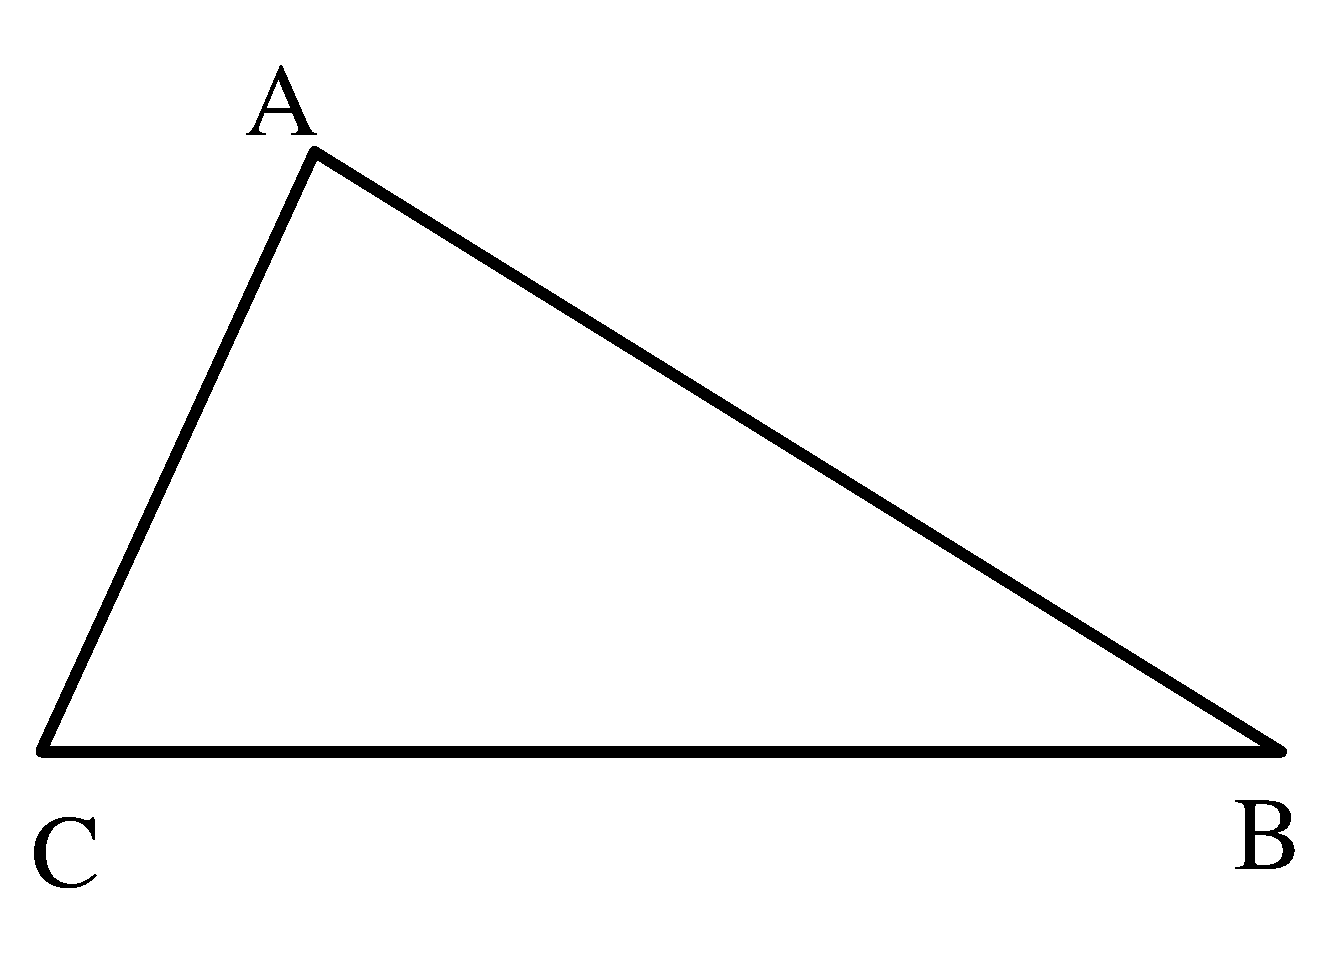
\includegraphics[keepaspectratio, width=3.0cm,height=2.4cm,clip]{eikaku_C.pdf}

                    (A) 鋭角三角形
                \end{center}
            \end{minipage}
            \begin{minipage}{0.5\hsize}
                \begin{center}
                    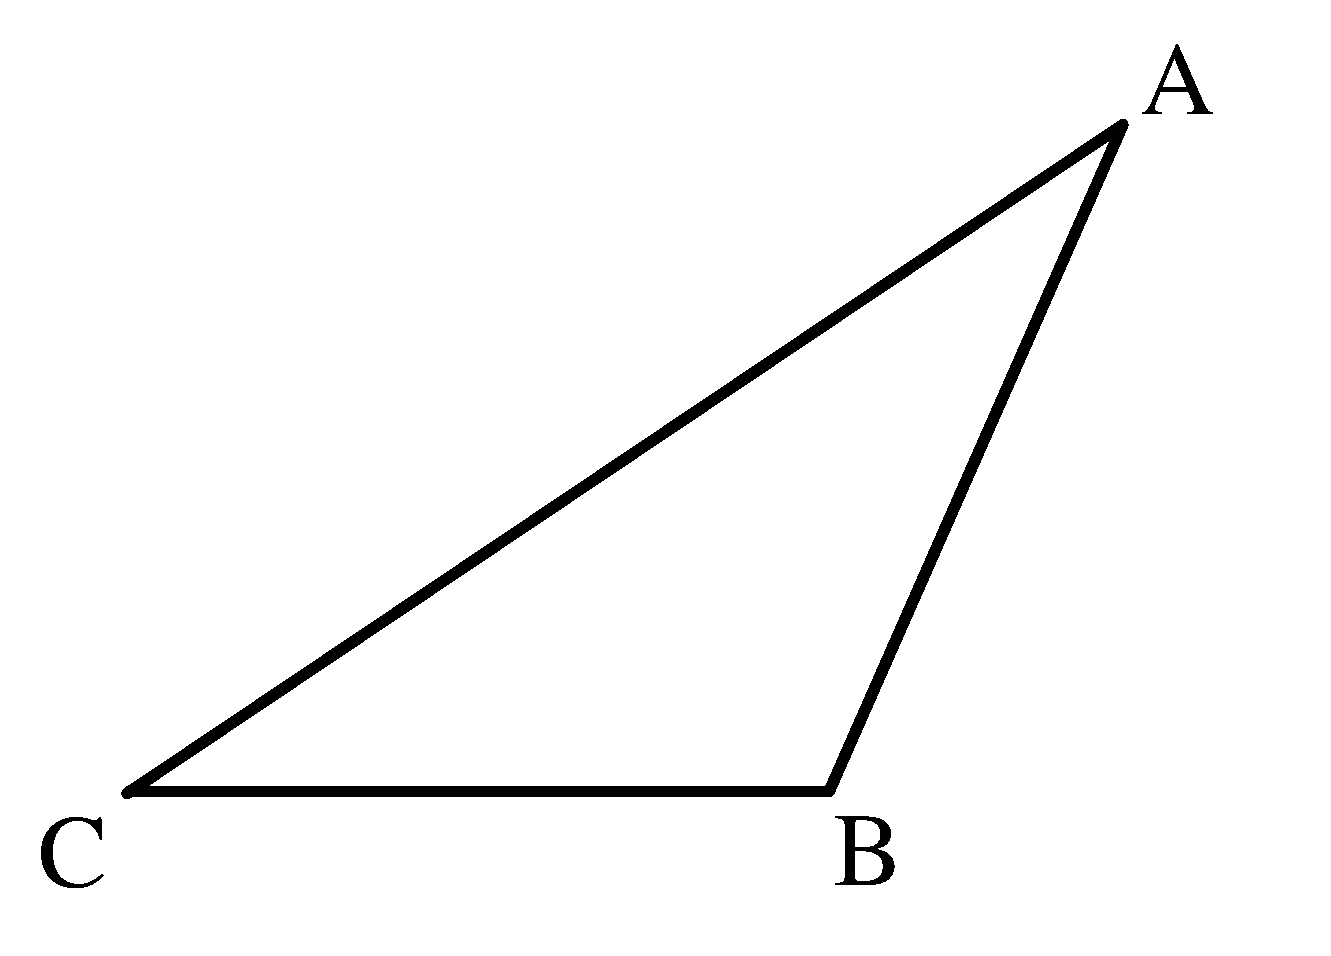
\includegraphics[keepaspectratio, width=3.0cm,height=2.4cm,clip]{donkaku_S.pdf}

                    (B) 鈍角三角形
                \end{center}
            \end{minipage}
        \end{tabular}
        \label{fig:sankakukei_no_katati}
        \caption{三角形の種類}
    \end{figure}

    ここで確認したいのは,$\sin$ 関数と $\cos$ 関数である.
    図の三角形(鋭角,鈍角のどちらでもよい)で,三角形の頂点Aから,辺BCもしくはその延長に
    対して垂線を引く.垂線の足
        \footnote{
            垂線の足:頂点Aから辺BCの延長の交点のこと.
        }
    を $H$ とする.$\angle \mathrm{ABC}$ の角度を $\theta$ と表す.
    \begin{figure}[hbt]
        \begin{tabular}{cc}
            \begin{minipage}{0.5\hsize}
            \begin{center}
                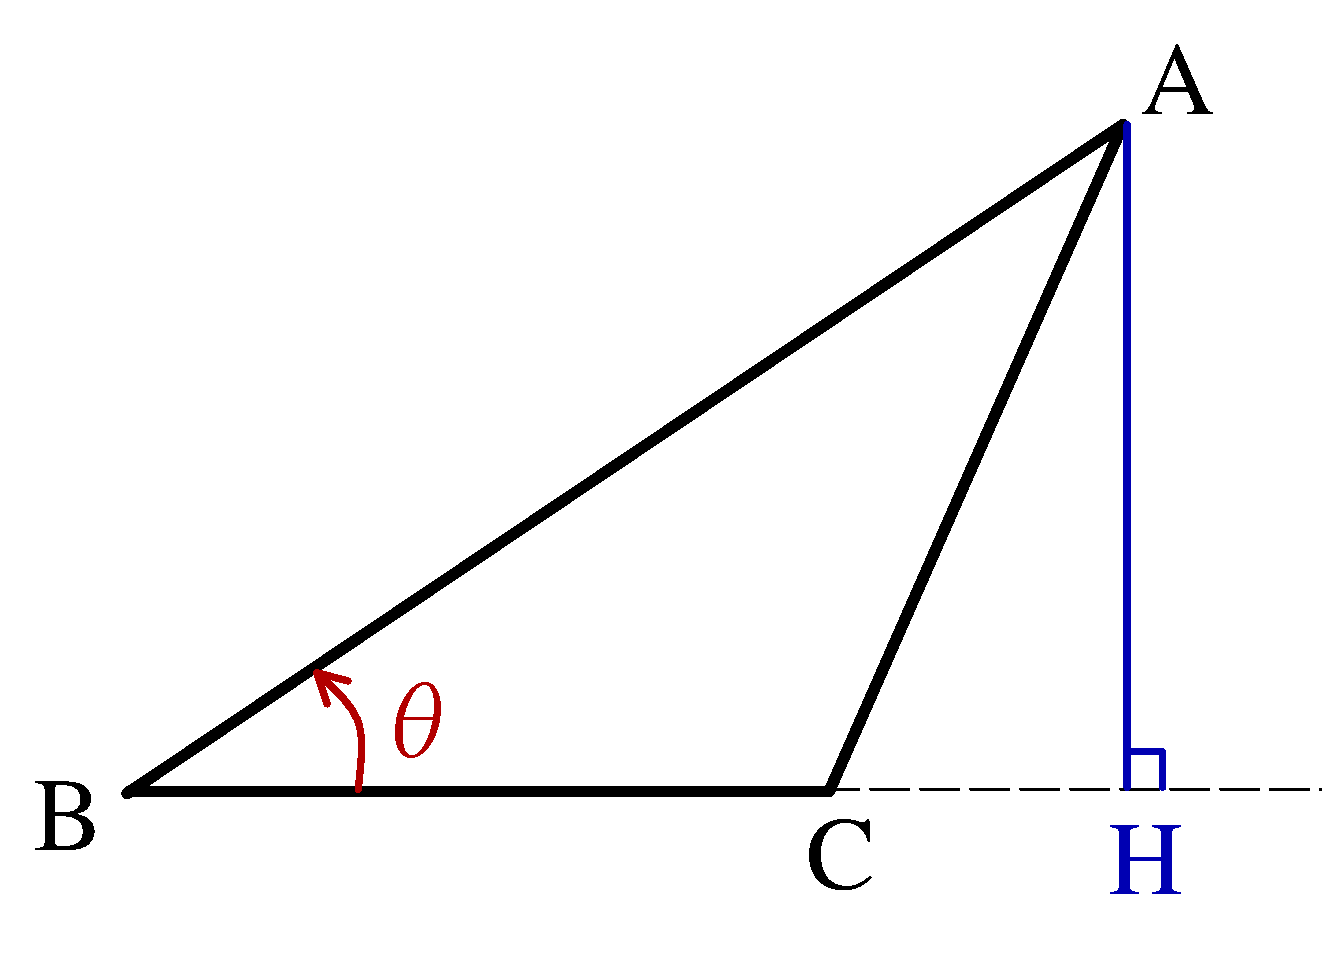
\includegraphics[keepaspectratio, width=3.5cm,height=2.8cm,clip]{function_sin_1.pdf}

                (A)
            \end{center}
            \end{minipage}
            \begin{minipage}{0.5\hsize}
            \begin{center}
                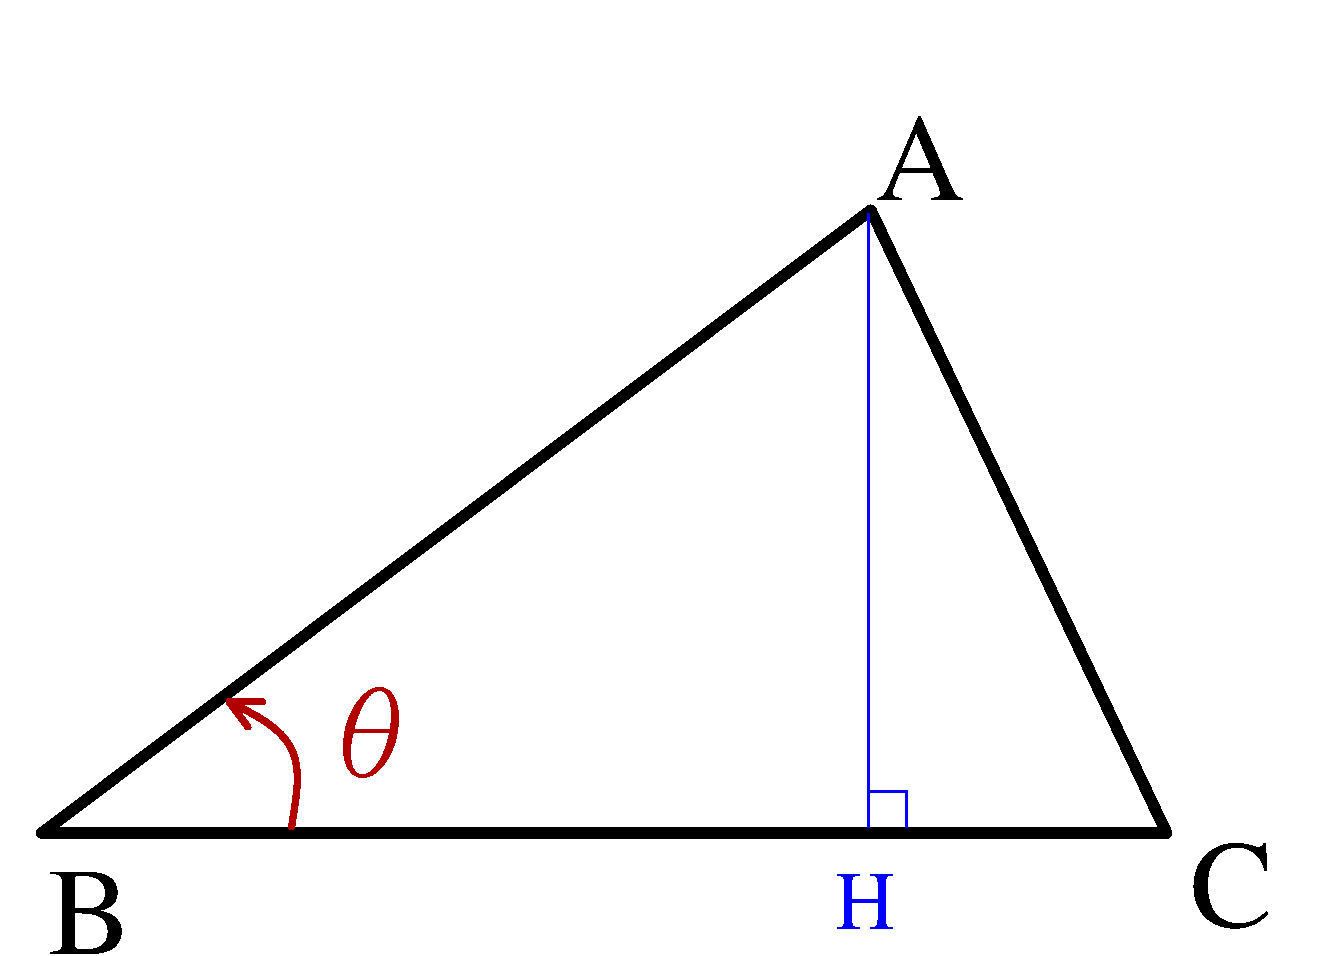
\includegraphics[keepaspectratio, width=3.5cm,height=2.8cm,clip]{function_sin_2.pdf}

                (B)
            \end{center}
            \end{minipage}
        \end{tabular}
        \caption{垂線の引き方}
        \label{fig:suisen_no_hikikata}
    \end{figure}

    これから大事なるのが,垂線AHとBHである.
    つまり,直角三角形を考えることになる.
    三角比には一般の三角形で成り立つような,
    「正弦定理」や「余弦定理」などがあるが,これらはここでは
    考えず,必要になった時に確認するという形にしたい.
    とりあえずは直角三角形を考える.

    ということで,図を以下のように書き直そう.
        \begin{figure}[hbt]
            \begin{center}
                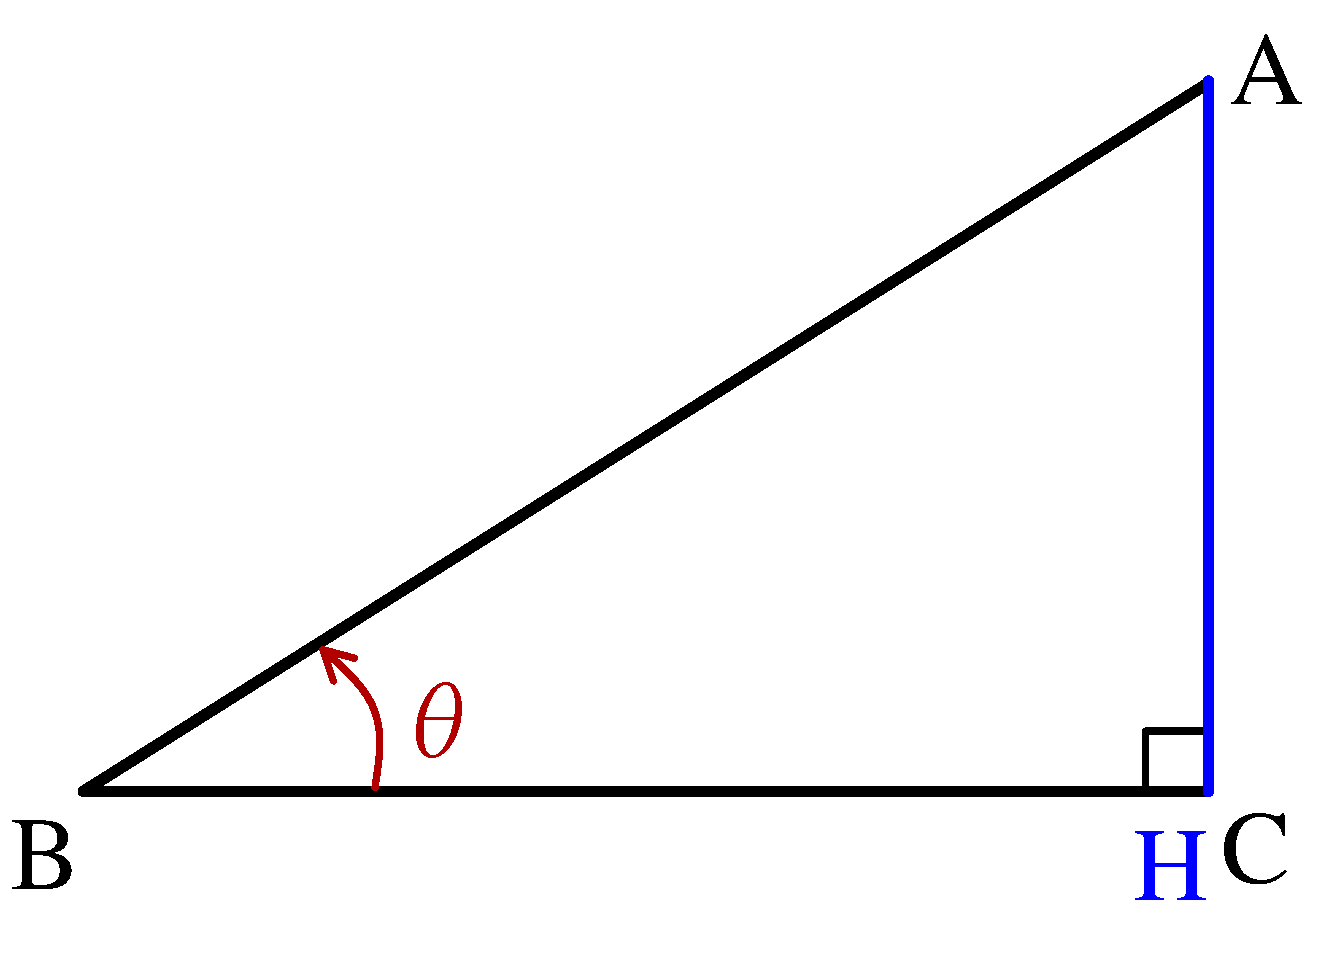
\includegraphics[keepaspectratio, width=3.5cm,height=2.8cm,clip]{sincos111.pdf}
                \caption{直角三角形の図}
                \label{fig:sincos111}
            \end{center}
        \end{figure}

    直角三角形は,辺ABの長さ $\|\mathrm{AB}\|$ と角度 $\theta$ で,その形を特定できる.
        \footnote{
            言い換えると,$\|\mathrm{AB}\|$ と $\theta$ の2つが特定されると,
            三角形の形とその大きさがきまる,ということ.
        }
    つまり,$\|\mathrm{AB}\|$ と $\theta$ がそれぞれ
    1つずつ定まれば,垂線AHの長さ $\|\mathrm{AH}\|$ が1つに定まるという関係がある.
    従って,$\|\mathrm{AH}\|$ は,$\|\mathrm{AB}\|$ と $\theta$ の関数であり,
        \begin{equation*}
            \|\mathrm{AH}\| = \|\mathrm{AB}\|\sin \theta
        \end{equation*}
    と表現する.辺ABが,基準となる水平な線よりも角度 $\theta$ だけ傾いている
    ときの,縦方向の長さが $\|\mathrm{AH}\|$ なのである.
    \begin{figure}[hbt]
        \begin{tabular}{cc}
            \begin{minipage}{0.5\hsize}
            \begin{center}
                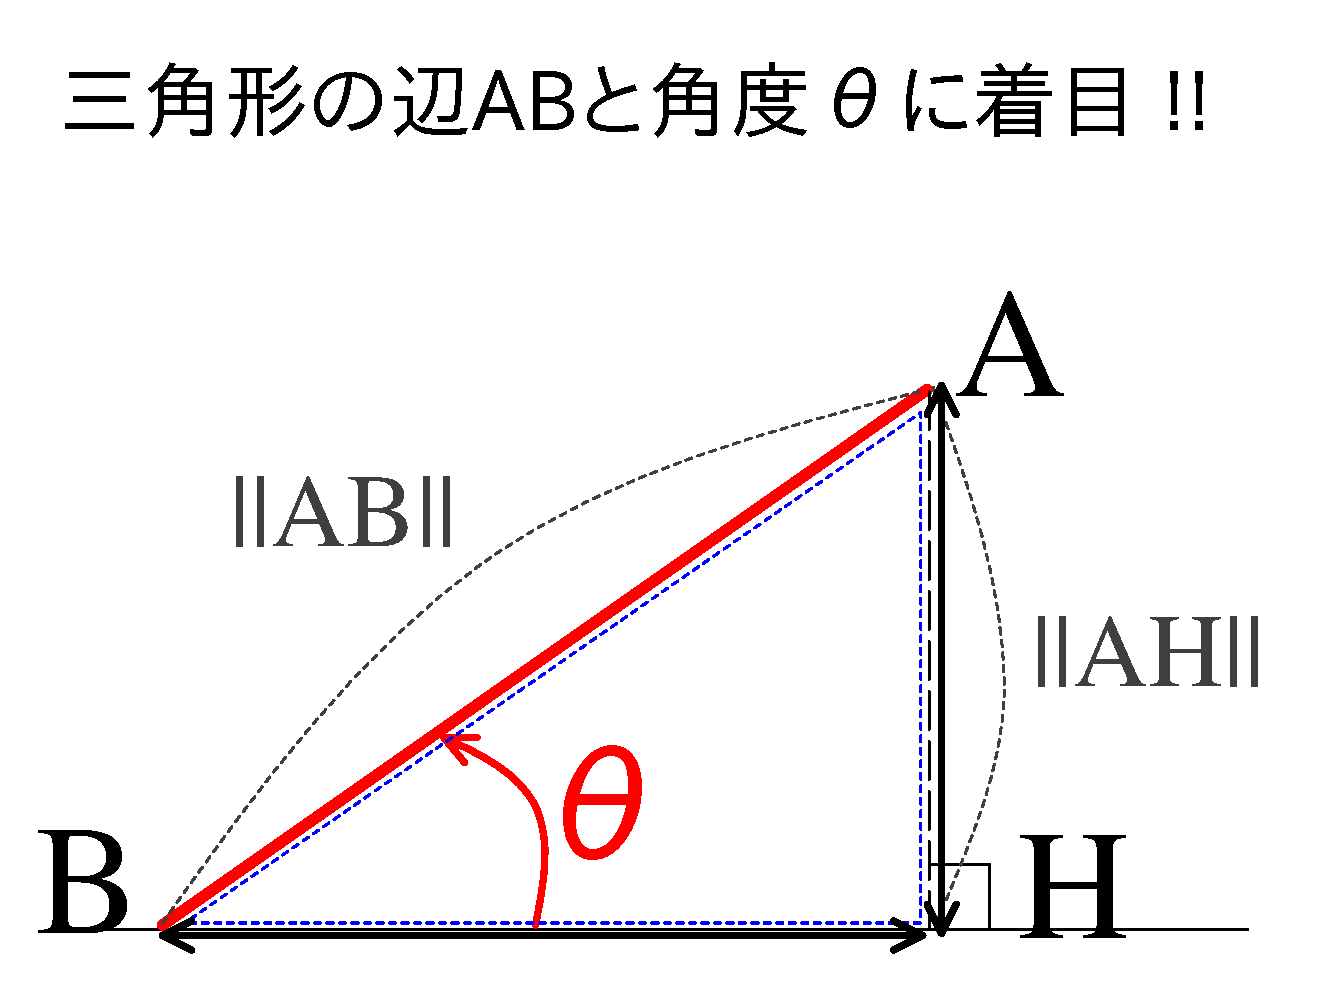
\includegraphics[keepaspectratio, width=3.5cm,height=2.8cm,clip]{sankakuhi-ABH.pdf}

                (A)
            \end{center}
            \end{minipage}
            \begin{minipage}{0.5\hsize}
            \begin{center}
                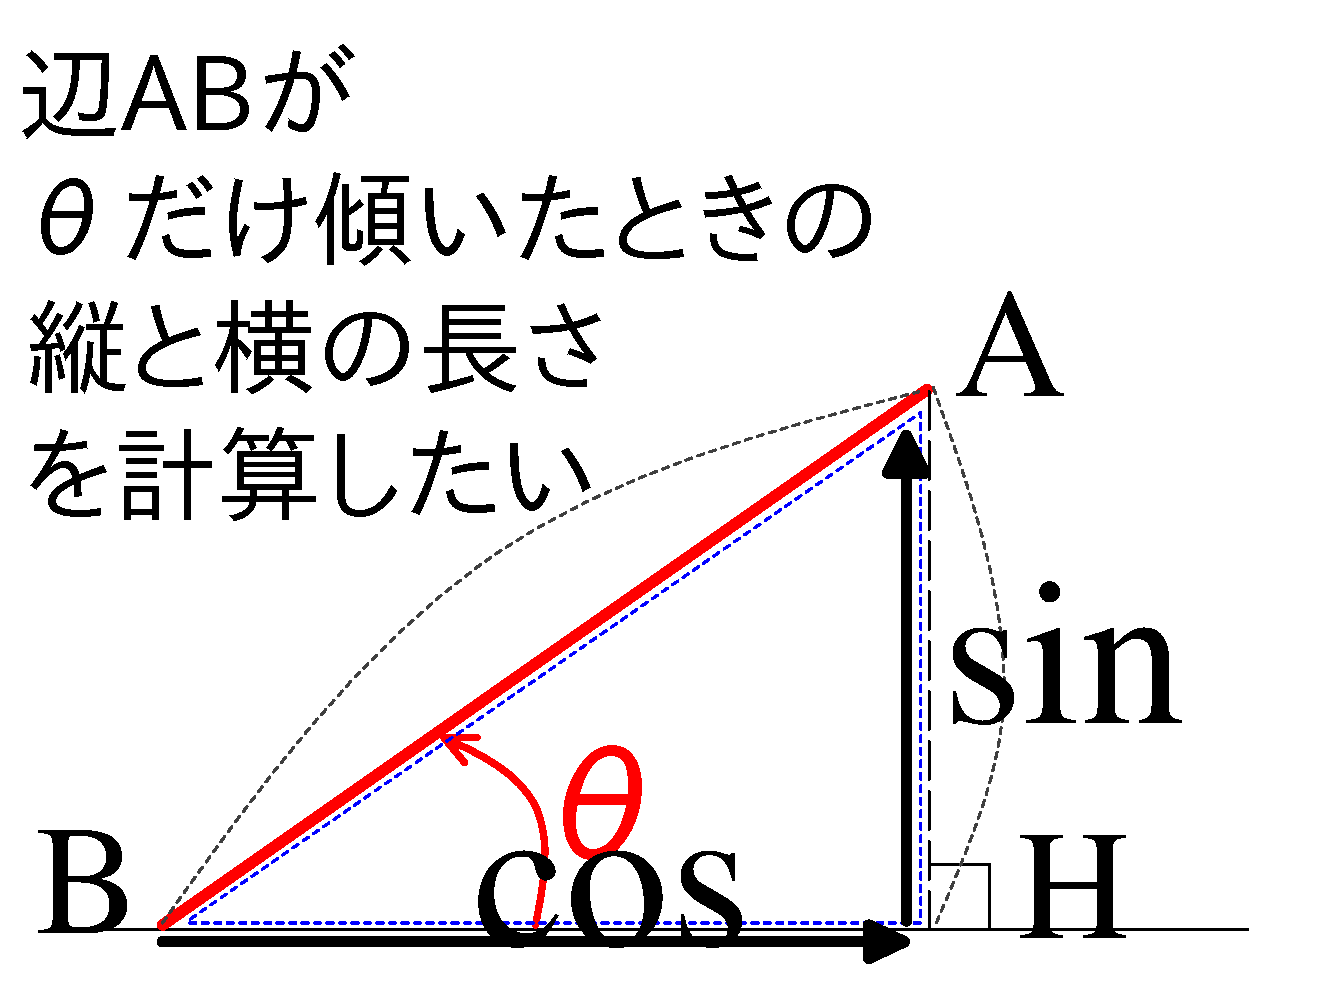
\includegraphics[keepaspectratio, width=3.5cm,height=2.8cm,clip]{sankakuhi-ABH-2.pdf}

                (B)
            \end{center}
            \end{minipage}
        \end{tabular}
        \caption{三角形の見方を変えよう}
        \label{fig:sankakukei-no-mikata}
    \end{figure}

    もう一方の辺BHの長さ $\|\mathrm{BH}\|$ も,$\|\mathrm{AB}\|$ と $\theta$ の関数である.
        \begin{equation*}
            \|\mathrm{BH}\| = \|\mathrm{AB}\|\cos \theta
        \end{equation*}
    と表現する.

    要するに,辺ABが $\theta$ だけ傾いている直角三角形の,
    縦の長さ($\|\mathrm{AH}\|$)が知りたい場合,$\|\mathrm{AB}\|$ に $\sin \theta$ を
    かけて,
        \begin{equation*}
            \|\mathrm{AH}\| = \|\mathrm{AB}\| \sin \theta
        \end{equation*}
    と計算できるということだ.横の長さ($\|\mathrm{BH}\|$)を知りたければ,$\cos \theta$ をかければよく,
        \begin{equation*}
            \|\mathrm{BH}\| = \|\mathrm{AB}\| \sin \theta
        \end{equation*}
    と計算される.$\sin \theta$ と $\cos \theta$ の値は,すでに先人が計算していて,
    今では,三角関数の表として,簡単に参照できるし,$\|\mathrm{AB}\|$ もわかる.
    つまり,三角関数を使うことで,辺ABとその傾射ている角度 $\theta$ から,
    縦と横の長さを計算で出すことができるのだ.

    さらに,$\sin \theta$ と $\cos \theta$ を使うと,
    辺ABの傾きを表現できる.一次関数,
    つまり直線の式
    では,$y=ax+b$ の $a$ が
    直線 $y$ の傾きを表している.
    傾きとは,
        \begin{equation*}
            a=\frac{(y\mbox{の増加量})}{(x\mbox{の増加量})}
        \end{equation*}
    で定義される量であった.この式の分母に $\|\mathrm{AB}\|\cos\theta$を,
    分子に $\|\mathrm{AB}\|\sin\theta$ を入れると,
        \begin{equation*}
            \frac{\sin\theta}{\cos\theta}
        \end{equation*}
    である.($\|\mathrm{AB}\|$ は約分される.)
    これは,辺ABの傾きにほかならない.これを,$\tan$ という関数記号を
    導入し,
        \begin{equation*}
            \tan\theta =\frac{\sin\theta}{\cos\theta}
        \end{equation*}
    と表現する.三角比には他にもいろいろな公式があるが,ここでは省略する.
    三角比は三角関数の特殊($0^{\circ}< \theta <180^{\circ}$)な例である.
    従って,三角比の公式は,三角関数でも成り立つ.三角関数を説明した後,
    そのうちの重要な公式を確認しよう.

    では次に,三角関数にとりかかろう.

\subsubsection{三角関数の定義}
    三角関数の定義する
        \footnote{
            この定義は,図形を用いてなされるので,
            かなり直観的で,何か受け入れがたい
            のだが,とりあえず便宜上の定義として
            考えてもらいたい.しかし,この定義は
            完全に間違っているわけではない.
            図形的に定義されるから,そこに直観が入り,
            論理が崩れてしまうという恐れがあるだけである.
            このノートでは,この図形的定義で十分である.
        }.
    図\ref{fig:sankakukansu1}を参照してほしい.
        \begin{figure}[hbt]
            \begin{center}
                \includegraphicsdefault{sankakukansu1.pdf}
                \caption{三角関数}
                \label{fig:sankakukansu1}
            \end{center}
        \end{figure}

    図を見るときに,半径 $r$ の円上を回転
    しているイメージしてほしい.この回転により,$\theta$ がいろいろな値
    に変化している様子が想像できればよい.${0\,}^{\circ} < \theta < {360\,}^{\circ}$ に
    \textbf{限らず},何回転でもできる.また,右回転(図\ref{fig:sankakukansu1}の矢印の向き)を
    正方向の回転として,その逆回転の負方向の回転も可能である.負の回転の場合,$\theta$ の取りうる
    値は負になる.この回転する半径のことを,\textbf{動径} とよぶ.\\

        \begin{itembox}[l]{三角関数の定義}
            図\ref{fig:sankakukansu1}において,三角関数 $\sin\theta$,
            $\cos\theta$,$\tan\theta$ を次で定義する.
                \begin{align}
                    \sin\theta := \frac{y}{r}\\ \notag \\
                    \cos\theta := \frac{x}{r}\\ \notag \\
                    \tan\theta := \frac{y}{x}
                \end{align}
        \end{itembox}\\
    $r$ は円の半径である.この定義では,もちろん $r  \neq  0$ と仮定している.

\subsubsection{三角関数の図形的イメージ}
    三角関数の定義式を見ても,最初はイメージしにくいここと思う.
    だから,ここで,三角関数の図形的イメージを押さえておこう.

    \begin{mysmallsec}{$\cos$ 関数のイメージ}
        最初に,$\cos$ 関数のイメージを考える.$\cos$ 関数の定義式は
            \begin{equation*}
                \cos \theta = \frac{x}{r}
            \end{equation*}
        である.但し,右辺は直交座標による.$r$ は円の半径であるから,
        定数として見てよい.例えば,$r=1$ の場合を考えてみよう.$r=1$ の
        場合,定義式により
            \begin{equation*}
                \cos \theta = x
            \end{equation*}
        となる.これは何を表しているか.式の示す通りである.
        $\cos \theta$ は $x$ の座標値に等しい.三角形で考えれば,
        半径 $r$ を斜辺とみなしたときの,$x$ 座標に等しいのである.


        半径が1でない場合はどうだろうか.その場合,定義式から,
            \begin{equation*}
                r \cos \theta = x
            \end{equation*}
        である.単に半径が1の場合の $r$ 倍になったにすぎない.


        これは,半径の $x$ 方向だけを考えたい場合に便利な道具となる.
        動径はいろいろな角度に運動するだろうが,その方向全てではなく,
        $x$ 軸方向のみを知りたい場合,その時の動径の角度を $\theta$ と
        して,$\cos \theta$ をかければよいのだ.


        長さ $r$ をもつ動径が,角度 $\theta$ の位置にあるとき,その時の
        $x$ 座標は $x = r \cos \theta$ で計算できる.半径 $r$ に $\cos \theta$ を
        かけると $x$ 座標が分かるのである.

        これはまた,\textbf{動径の $x$ 方向の長さを示している}とみても同じことである.
    \end{mysmallsec}


    \begin{mysmallsec}{$\sin$ 関数のイメージ}
        $\sin$ 関数も,$\cos$ 関数と同じように考えられる.
        $\sin$ 関数の定義は
            \begin{equation*}
                \sin \theta = \frac{y}{r}
            \end{equation*}
        である.
        半径 $r = 1$ の場合,それは動径の $y$ 座標を示す.
        $r\neq1$ の場合は,
            \begin{equation*}
                r \sin \theta = y
            \end{equation*}
        である.これは動径の $y$ 座標に他ならない.
        動径の $x$ 座標を知りたい場合は,半径に $\cos \theta$ を
        かければよいのと同様に,動径の $y$ 座標を知りたい場合は,
        $\sin \theta$ を半径 $r$ にかければよい.

        長さ $r$ をもつ動径が,角度 $\theta$ の位置にあるとき,その時の
        $y$ 座標は $y = r \sin \theta$ で計算できる.半径 $r$ に $\sin \theta$ を
        かけると $y$ 座標が分かるのである.

        これはまた,\textbf{動径の $y$ 方向の長さを示している}とみても同じことである.
    \end{mysmallsec}


    \begin{mysmallsec}{$\tan$ 関数のイメージ}
        では,$\tan$ 関数は同イメージされるのだろう.
        $\tan$ 関数の定義は
            \begin{equation*}
                \tan \theta = \frac{y}{x}
            \end{equation*}
        である.
        定義そのものを見れば,答えは意外に簡単だ.
        動径の傾きを表しているのである.これは定義式から明らかだ.動径の
        一端は常に座標のある一点から動かない.今の場合は,
        考えやすいように,座標原点に一端を固定している.だから,
            \begin{equation*}
                \frac{y}{x} = \frac{y-0}{x-0}
            \end{equation*}
        と見ることができる.動径の回転中心が座標原点ではなく,
        $(\,x_{0},\,y_{0}\,)$ の場合は
            \begin{equation*}
                \frac{y-y_{0}}{x-x_{0}}
            \end{equation*}
        である.どちらの場合も,
            \begin{equation*}
                \frac{y\mbox{の増加量}}{x\mbox{の増加量}}
            \end{equation*}
        と見ることができる.

        \textbf{$\tan$ は,動径を一次関数と見立てた時の,変化の割合を示す量}と
        見ることができる.
    \end{mysmallsec}

\subsubsection{三角関数の性質}
    三角関数には公式がいろいろとある.ここでいくつかを
    確認しておこう.

    まず,三平方の定理から,\\

        \begin{itembox}[l]{三角関数の公式}
            \begin{align}
                \sin^{2} \theta  +  \cos^{2} \theta  =  1
            \end{align}
        \end{itembox}\\
    が成立する.

    \begin{mysmallsec}{説明}
        簡単に説明する.直交座標において,
            \begin{equation*}
                x^{2}  +  y^{2}  =  r^{2}
            \end{equation*}
        が成立する.さて,この $x$,$y$ は三角関数の定義から,
            \begin{equation*}
                x  =   r \cos \theta \quad, \quad y  =  r \sin \theta
            \end{equation*}
        である.つまり,
            \begin{align*}
                x^{2}  +  y^{2}  &=  r^{2} \\
                (r \cos \theta)^{2}  +  (r \sin \theta)^{2}  &=  r^{2} \\
                r^{2} \cos^{2} \theta  +  r^{2} \sin^{2} \theta  &=  r^{2}.
            \end{align*}
        $r\neq0$ だから $r^{2} \neq 0$ であり,$r^{2}$ で割ると,
            \begin{equation*}
                \sin^{2} \theta  +  \cos^{2} \theta  =  1
            \end{equation*}
        が導かれる.
    \end{mysmallsec}


